\documentclass[notes,blackandwhite,mathsans]{beamer}

\usepackage{amsmath}
\usepackage{amssymb}
\usepackage{graphicx}
\usepackage{fancybox}
\usepackage{booktabs}
\usepackage{multirow,pxfonts}
\usepackage{cmbright}
\usepackage{color}
\usepackage{xcolor}
\usepackage{enumitem}
\usepackage{changepage}

\usepackage[T1]{fontenc}
\fontencoding{T1}  
\usepackage[utf8]{inputenc}


\usefonttheme{default}
\setbeamercovered{invisible}
\beamertemplatenavigationsymbolsempty

\makeatletter
\setbeamertemplate{footline}
{
  \leavevmode
  \hbox{
  \begin{beamercolorbox}[wd=0.97\paperwidth,ht=2.25ex,dp=2ex,right]{}
{\color{mcxs2} \insertframenumber{} / \inserttotalframenumber}
  \end{beamercolorbox}}%
}



\definecolor{mcxs1}{HTML}{05386B}
\definecolor{mcxs2}{HTML}{379683}
\definecolor{mcxs3}{HTML}{5CDB95}
\definecolor{mcxs4}{HTML}{8EE4AF}
\definecolor{mcxs5}{HTML}{EDF5E1}
\setbeamercolor{frametitle}{fg=mcxs2}
\AtBeginDocument{\color{mcxs1}}

%\setbeamercolor{itemize text}{fg=mcxs5}
\setbeamercolor{itemize item}{fg=mcxs1}
\setbeamercolor{itemize subitem}{fg=mcxs2}
\setbeamercolor{enumerate item}{fg=mcxs1}
\setbeamercolor{description item}{fg=mcxs1}

\setbeamertemplate{itemize item}[triangle]
\setbeamertemplate{itemize subitem}[circle]




\begin{document}
%\fontfamily{pag}\selectfont
%\setbeamerfont{title}{family=\fontfamily{pag}\selectfont}
%\setbeamerfont{frametitle}{family=\fontfamily{pag}\selectfont}
%\setbeamerfont{framesubtitle}{family=\fontfamily{pag}\selectfont}







{\setbeamercolor{background canvas}{bg=mcxs1}
\begin{frame}

\vspace{1cm}
\begin{tabular}{rl}
&\textbf{\LARGE\color{mcxs2} Macroeconometrics}\\[8ex]
\textbf{\Large\color{mcxs2} Lecture 3}&\textbf{\Large\color{mcxs3}Bayesian Estimation}\\[19ex]
&\textbf{\color{mcxs2} Tomasz Wo\'zniak}\\[1ex]
&{\small\color{mcxs3} Department of Economics}\\
&{\small\color{mcxs3}University of Melbourne}
\end{tabular}

\end{frame}
}



{\setbeamercolor{background canvas}{bg=mcxs1}
\begin{frame}

\vspace{0.5cm} \textbf{\color{mcxs3}Bayes' rule}

\bigskip\textbf{\color{mcxs2}Useful distributions}

\bigskip\textbf{\color{mcxs2}Likelihood function}

\bigskip\textbf{\color{mcxs2}Prior distribution}

\bigskip\textbf{\color{mcxs2}Posterior distribution}



\vspace{0.5cm}{\color{mcxs5}Readings:} \\ \footnotesize
{\color{mcxs2}Wo\'zniak (2021) Posterior derivations for a simple linear regression model, Lecture notes}\\
\smallskip{\color{mcxs2}Greenberg (2008) Chapter 4: Prior Distributions, Introduction to Bayesian Econometrics}

\bigskip\normalsize{\color{mcxs5}Materials:}\\ \footnotesize
{\color{mcxs2}An R file} \texttt{\color{mcxs5}L3 grphs.R} {\color{mcxs2}for the reproduction of graphs}\\
%{\color{mcxs2}Selected quotations from Sims (2012) -- Bayesian vs. frequentist approach}

\end{frame}
}



%{\setbeamercolor{background canvas}{bg=mcxs2}
%\begin{frame}
%
%\bigskip\textbf{\color{mcxs1}Objectives.}
%\begin{itemize}[label=$\blacktriangleright$]
%\item {\color{mcxs1}To learn the basics of Bayesian inference}
%\item {\color{mcxs1}To familiarise with essential probability distributions}
%\item {\color{mcxs1}To derive Bayesian estimation results for a simple model}
%\end{itemize}
%
%\bigskip\textbf{\color{mcxs3}Learning outcomes.}
%\begin{itemize}[label=$\blacktriangleright$]
%\item {\color{mcxs3}Using basic Bayesian terminology}
%\item {\color{mcxs3}Identifying parameters of transformed distributions}
%\item {\color{mcxs3}Recognising functional form of kernels of basic distributions}
%\end{itemize}
%
%\end{frame}
%}





\begin{frame}

\centering
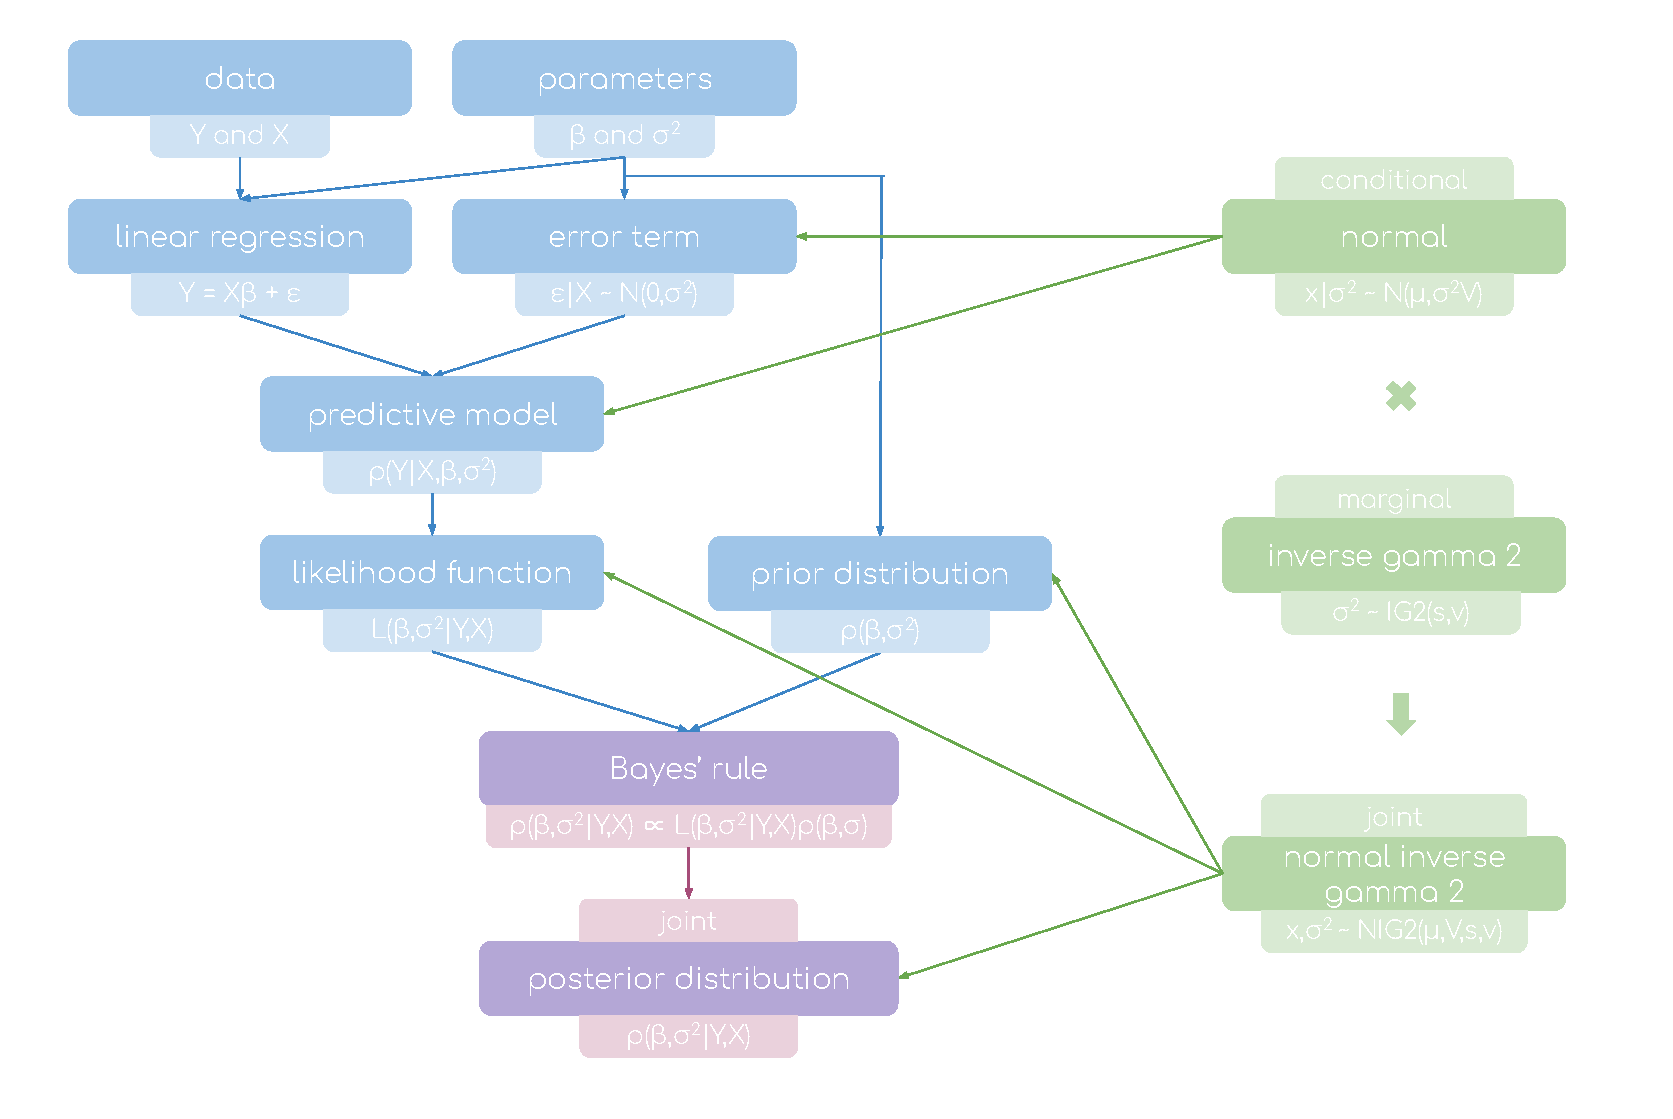
\includegraphics[scale=0.45, trim= 1.8cm 2cm 2cm 0.5cm]{grphs/03conceptmap.pdf}

\end{frame}




\begin{frame}

\centering
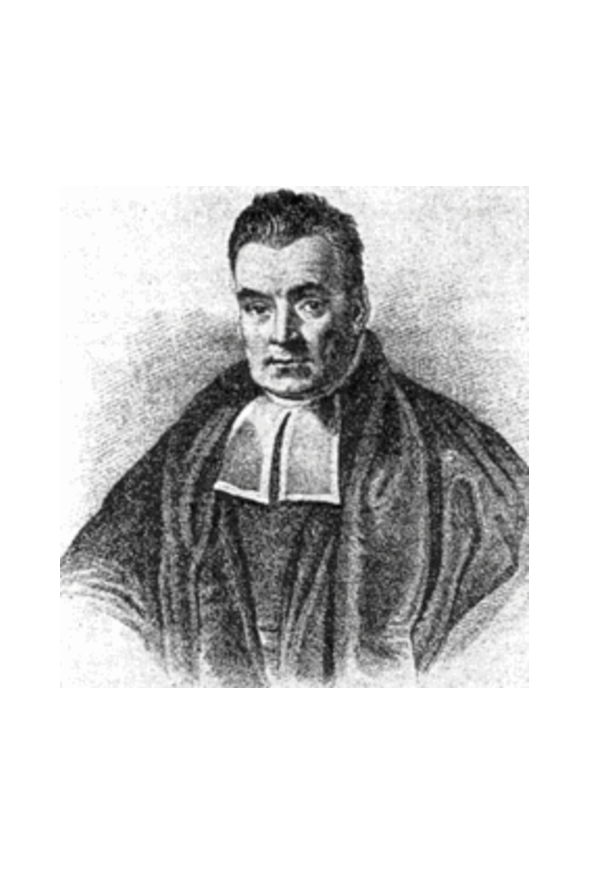
\includegraphics[scale=0.5, trim= 2cm 2cm 2cm 2cm]{grphs/Bayes.pdf}

\Large\textbf{\color{mcxs3} Bayes'} \textbf{\color{mcxs2}rule}

\end{frame}





\begin{frame}
\frametitle{Bayes' rule}

$$ p\left( \theta|Y \right) = \frac{p\left( Y|\theta \right)p\left( \theta \right)}{p\left( Y \right)}  $$

%\small

\bigskip
\begin{description}
\item[$p\left( \theta|Y \right)$] {\color{mcxs2}- posterior distribution of parameters} $\theta$ {\color{mcxs2}given data} $Y$
\item[$p\left( Y|\theta \right)$] {\color{mcxs2}- sampling distribution of data} $Y$ {\color{mcxs2}given parameters} $\theta$
\item[$p\left( \theta \right)$] {\color{mcxs2}- prior distribution of parameters} $\theta$
\item[$p\left( Y \right)$] {\color{mcxs2}- marginal data density}
\end{description}

\end{frame}


\begin{frame}
\frametitle{Bayes' rule}

$$ p\left( \theta|Y \right) \propto L\left( \theta| Y \right)p\left( \theta \right)$$

%\small
\bigskip
\textbf{Learning mechanism.}

{\color{mcxs2}The prior information about the parameters is updated by the information contained in the data and represented by the likelihood function resulting in the posterior distribution.}

\bigskip
\textbf{Likelihood principle.}

{\color{mcxs2}All the information about the parameters of the model included in the data is captured by the likelihood function.}

\end{frame}


{\setbeamercolor{background canvas}{bg=mcxs1}
\begin{frame}
\frametitle{Bayes' rule}

\centering
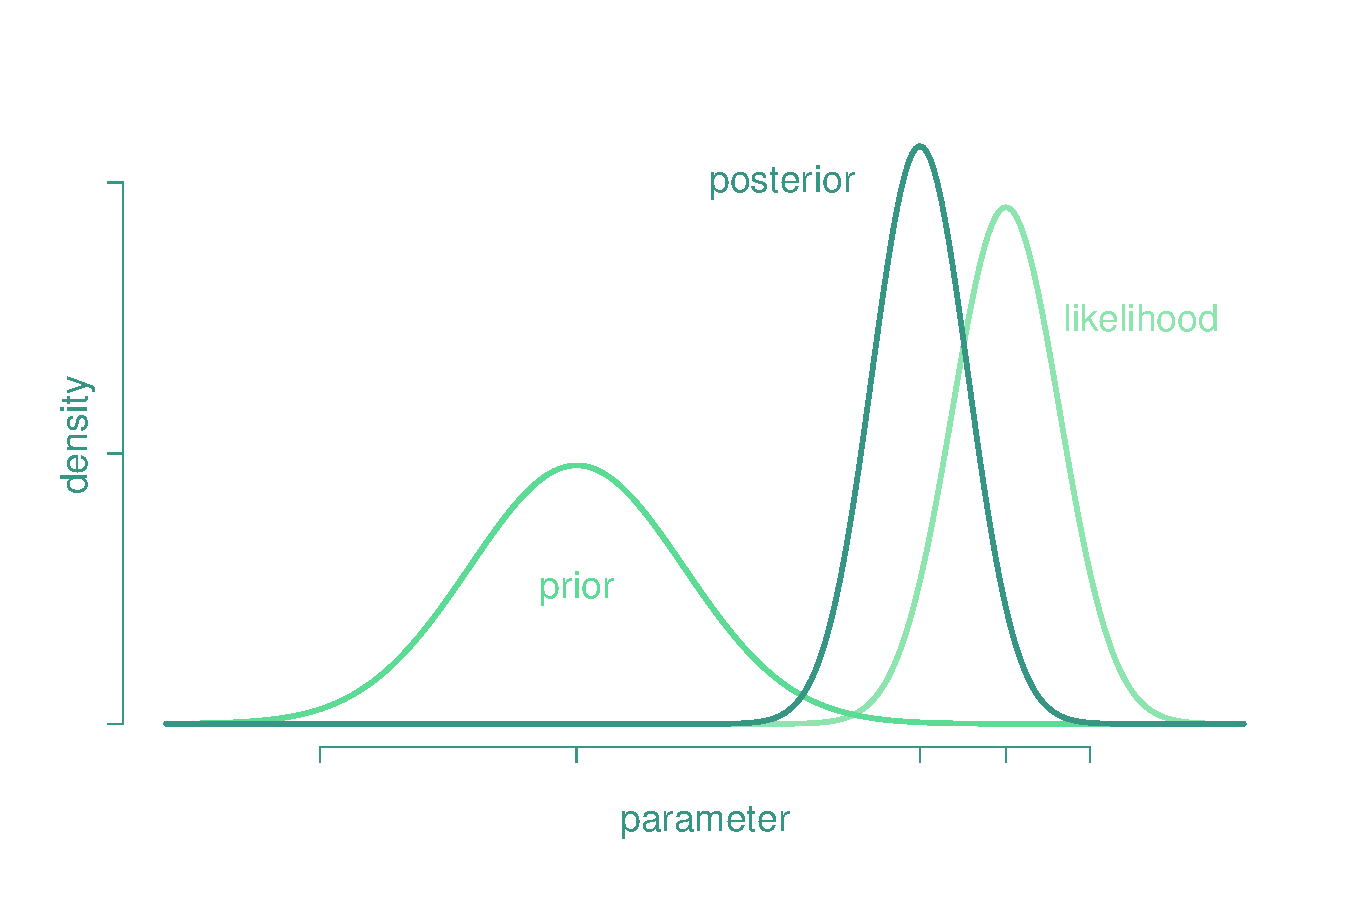
\includegraphics[scale=0.45]{grphs/learning.pdf}

\end{frame}
}




{\setbeamercolor{background canvas}{bg=mcxs1}
\begin{frame}
\frametitle{Bayes' rule}

\centering
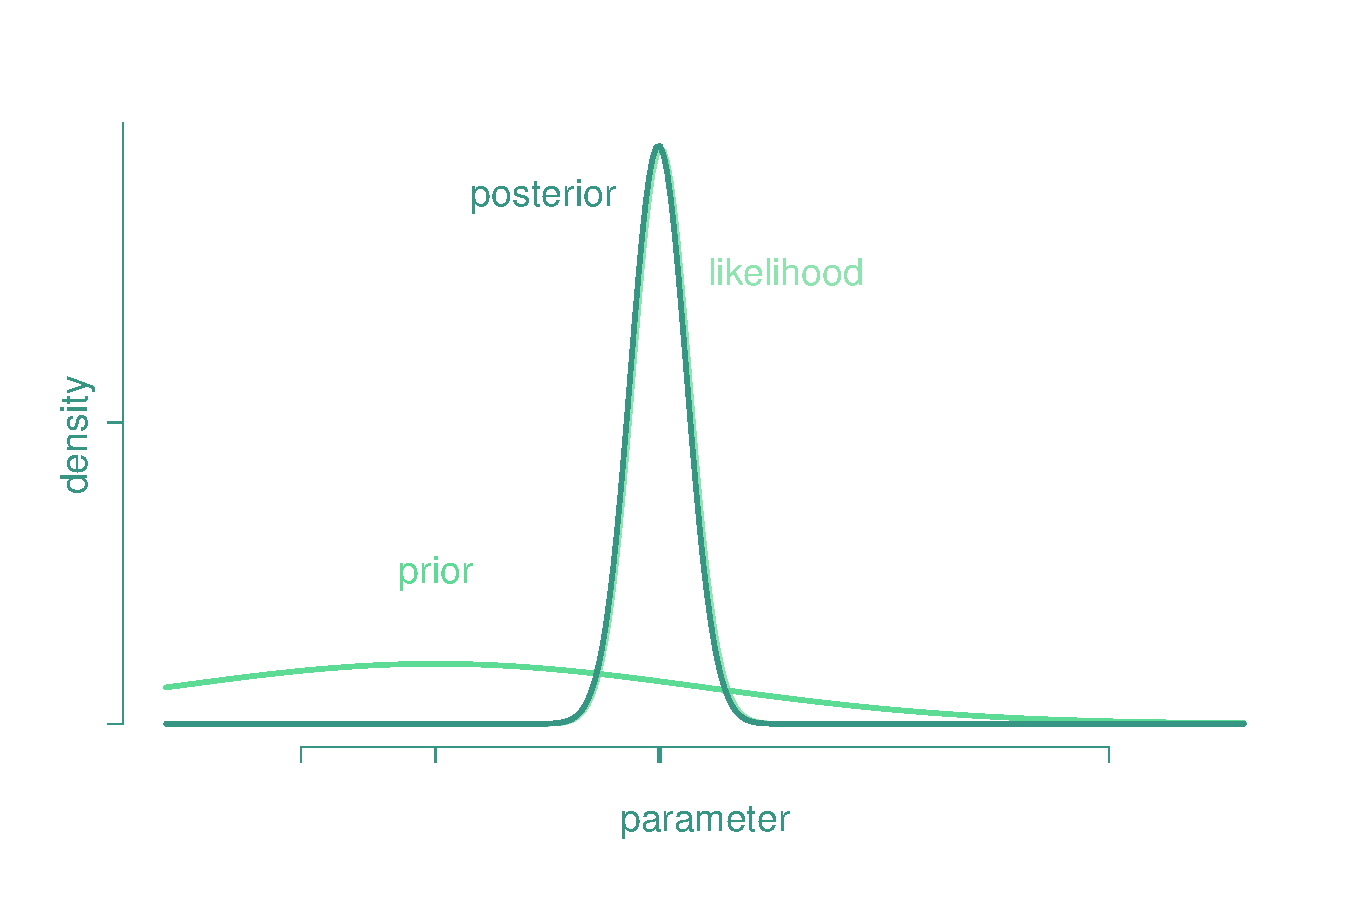
\includegraphics[scale=0.45]{grphs/learning_better.pdf}

\end{frame}
}




\begin{frame}
\frametitle{Bayes' rule}

\textbf{Joint distribution of data and parameters.}

$$ p\left( Y|\theta \right)p\left( \theta \right) = p\left( Y, \theta \right) =  p\left( \theta|Y \right)p\left( Y \right) $$

\vspace{1cm}{\color{mcxs2}The joint distribution of data and parameters is decomposed into:}

\begin{description}\small
\item[Inputs:] {\color{mcxs2}likelihood function} $p\left( Y|\theta \right)$ {\color{mcxs2}and prior distribution} $p\left( \theta \right)$
\item[Outputs:] {\color{mcxs2}posterior distribution} $p\left( \theta|Y \right)$ {\color{mcxs2}and marginal data density} $p\left( Y \right)$
\end{description}

\end{frame}




{\setbeamercolor{background canvas}{bg=mcxs2}
\begin{frame}

\begin{adjustwidth}{-0.5cm}{0cm}
%\FlushLeft
\vspace{8.3cm}\Large
\textbf{{\color{mcxs1}Useful} {\color{mcxs4}distributions}}
\end{adjustwidth}

\end{frame}
}


\begin{frame}
\frametitle{Multivariate normal distribution}

{\color{mcxs2}Let an} $N\times1$ {\color{mcxs2}real-valued random vector} ${\color{mcxs3}X}$ {\color{mcxs2}follow a multivariate normal distribution:}
$$ {\color{mcxs3}X}\sim\mathcal{N}_N(\mu,\Sigma) $$
{\color{mcxs2}with the mean vector} $\mu$ {\color{mcxs2}and the covariance matrix} $\Sigma$.

\bigskip\textbf{pdf.}
$$ \mathcal{N}_N(\mu,\Sigma) = {\color{mcxs2}(2\pi)^{-\frac{N}{2}}\det(\Sigma)^{-\frac{1}{2}}}\exp\left\{ -\frac{1}{2}({\color{mcxs3}X}-\mu)'\Sigma^{-1}({\color{mcxs3}X}-\mu) \right\} $$

\bigskip\small\textbf{Moments.}
$$ \mathbb{E}({\color{mcxs3}X})=\mu, \text{ and }Var({\color{mcxs3}X})=\Sigma $$
\end{frame}




\begin{frame}
\frametitle{Inverse gamma 2 distribution}
\small

{\color{mcxs2}Let a positive real-valued scalar random variable} ${\color{mcxs3}x}$ {\color{mcxs2}follow an inverse gamma 2 distribution:}
$$ {\color{mcxs3}x}\sim\mathcal{IG}2(s,\nu) $$
{\color{mcxs2}with the shape parameter} $\nu>0$ {\color{mcxs2}and the scale parameter} $s>0$.

\bigskip\textbf{pdf.}
$$ \mathcal{IG}2(s,\nu) = {\color{mcxs2}\Gamma\left(\frac{\nu}{2}\right)^{-1}\left(\frac{s}{2}\right)^{\frac{\nu}{2}}} {\color{mcxs3}x}^{-\frac{\nu+2}{2}}\exp\left\{ -\frac{1}{2}\frac{s}{{\color{mcxs3}x}} \right\}$$

\bigskip\textbf{Moments.}
\begin{align*}
\mathbb{E}({\color{mcxs3}x})&=\frac{s}{\nu-2}\text{\color{mcxs2}, for } \nu>2, \text{ }Var({\color{mcxs3}x})=\frac{2}{\nu-4}\left[\mathbb{E}({\color{mcxs3}x})\right]^2\text{\color{mcxs2}, for } \nu>4\\
mode &= \frac{s}{\nu+2}
\end{align*}

\end{frame}






\begin{frame}
\frametitle{Normal inverse gamma 2 distribution}
\small
\begin{align*}
p\left({\color{mcxs3}X}|{\color{mcxs3}\sigma^2}\right)&=\mathcal{N}_N\left( \mu, {\color{mcxs3}\sigma^2}\Sigma \right)\\
p\left({\color{mcxs3}\sigma^2}\right)&=\mathcal{IG}2(s,\nu)
\end{align*}
{\color{mcxs2}Then,} $({\color{mcxs3}X,\sigma^2})$ {\color{mcxs2}follow a normal inverse gamma 2 distribution:}
$$ p({\color{mcxs3}X,\sigma^2})= p({\color{mcxs3}X|\sigma^2})p({\color{mcxs3}\sigma^2}) =\mathcal{NIG}2_N\left(\mu, \Sigma, s,\nu \right) $$


\bigskip\textbf{pdf.}\footnotesize
\begin{align*} 
\mathcal{NIG}2\left(\mu, \Sigma, s,\nu \right) &= {\color{mcxs2}c_{nig2}^{-1}}  \left({\color{mcxs3}\sigma^2}\right)^{-\frac{\nu+N+2}{2}}\exp\left\{ -\frac{1}{2}\frac{1}{{\color{mcxs3}\sigma^2}}\left[ s+({\color{mcxs3}X}-\mu)'\Sigma^{-1}({\color{mcxs3}X}-\mu) \right]\right\}\\
{\color{mcxs2}c_{nig2}} &= {\color{mcxs2}\Gamma\left(\frac{\nu}{2}\right)\left(\frac{s}{2}\right)^{-\frac{\nu}{2}}(2\pi)^{\frac{N}{2}}\det(\Sigma)^{\frac{1}{2}}}
\end{align*} 

\smallskip\small\textbf{Moments.}\footnotesize
\begin{align*}
\mathbb{E}\left({\color{mcxs3}X}\right)&=\mu\text{\color{mcxs2}, for } \nu>1, \text{ }Var\left({\color{mcxs3}X}\right)=\frac{s}{\nu-2}\Sigma\text{\color{mcxs2}, for } \nu>2\\
\mathbb{E}\left({\color{mcxs3}\sigma^2}\right)&=\frac{s}{\nu-2}\text{\color{mcxs2}, for } \nu>2, \text{ }Var\left({\color{mcxs3}\sigma^2}\right)=\frac{2}{\nu-4}\left[\mathbb{E}\left({\color{mcxs3}\sigma^2}\right)\right]^2\text{\color{mcxs2}, for } \nu>4
\end{align*}
\end{frame}







\begin{frame}
\frametitle{Normal inverse gamma 2 distribution}

\bigskip\textbf{Kernel of the $\mathcal{NIG}2$ distribution.}\footnotesize

\smallskip\begin{equation*} 
\mathcal{NIG}2\left(\mu, \Sigma, s,\nu \right) \propto \left({\color{mcxs3}\sigma^2}\right)^{-\frac{\nu+N+2}{2}}\exp\left\{ -\frac{1}{2}\frac{1}{{\color{mcxs3}\sigma^2}}({\color{mcxs3}X}-\mu)'\Sigma^{-1}({\color{mcxs3}X}-\mu) \right\}\exp\left\{ -\frac{1}{2}\frac{s}{{\color{mcxs3}\sigma^2}}\right\}
\end{equation*} 

\end{frame}




\begin{frame}
\frametitle{Normal inverse gamma 2 distribution}

\bigskip\textbf{Generating random numbers from the $\mathcal{NIG}2$ distribution.}\small
\smallskip\begin{align*} 
p\left( {\color{mcxs3}\beta},{\color{mcxs3}\sigma^2} \right) &= p\left( {\color{mcxs3}\beta}|{\color{mcxs3}\sigma^2} \right)p\left( {\color{mcxs3}\sigma^2} \right)\\[2ex]
p\left( {\color{mcxs3}\beta}|{\color{mcxs3}\sigma^2} \right) &= \mathcal{N}\left(\mu, {\color{mcxs3}\sigma^2}\Sigma \right)\\
p\left( {\color{mcxs3}\sigma^2} \right) &= \mathcal{IG}2\left(s,\nu \right)
\end{align*} 

\bigskip\normalsize\textbf{To draw $S$ draws from the $\mathcal{NIG}2$ distribution...}\small
\begin{description}
\item[Step 1:] Draw independently $S$ draws from the $\mathcal{IG}2\left(s,\nu \right)$. Collect these draws in sequence $\left\{ \sigma^{2(s)} \right\}_{s=1}^{S}$
\item[Step 2:] For each $\sigma^{2(s)}$ sample a corresponding draw of $\beta^{(s)}$ from $\mathcal{N}\left(\mu, {\color{mcxs3}\sigma^{2(s)}}\Sigma \right)$
\item[Return:] $\left\{ \beta^{(s)},\sigma^{2(s)} \right\}_{s=1}^{S}$ as draws from the target distribution.
\end{description}
\end{frame}





{\setbeamercolor{background canvas}{bg=mcxs1}
\begin{frame}

\begin{adjustwidth}{-0.5cm}{0cm}
%\FlushLeft
\vspace{8.3cm}\Large
\textbf{{\color{mcxs2}Likelihood} {\color{mcxs5}function}}
\end{adjustwidth}

\end{frame}
}



\begin{frame}
\frametitle{Likelihood function}

\bigskip\textbf{A simple linear regression model.}
\begin{align*} 
Y &= \beta X + E\\
E|X &\sim\mathcal{N}\left(\mathbf{0}_T, \sigma^2I_T\right)\\
\downarrow &\\
Y|X &\sim\mathcal{N}\left(\beta X, \sigma^2I_T\right)
\end{align*} 

\bigskip\textbf{The likelihood function.}
\begin{equation*}
L\left(\theta|Y,X\right) = {\color{mcxs2}(2\pi)^{-\frac{T}{2}}} \left( {\color{mcxs3}\sigma^2} \right)^{-\frac{T}{2}}\exp\left\{ -\frac{1}{2}\frac{1}{\color{mcxs3}\sigma^2}(Y-{\color{mcxs3}\beta} X)'(Y-{\color{mcxs3}\beta} X) \right\}
\end{equation*}

\end{frame}




\begin{frame}
\frametitle{Likelihood function}

\textbf{The likelihood function as the $\mathcal{NIG}2$ distribution.}\footnotesize
\begin{align*}
L&\left(\theta|Y,X\right) \propto \left( \sigma^2 \right)^{-\frac{T}{2}}\exp\left\{ -\frac{1}{2}\frac{1}{\sigma^2}(Y-\beta X)'(Y-\beta X) \right\}\\[1ex]
&= \left( \sigma^2 \right)^{-\frac{T}{2}}\exp\left\{ -\frac{1}{2}\frac{1}{\sigma^2}(Y{\color{mcxs3}-\hat\beta X +\hat\beta X} - \beta X)'(Y{\color{mcxs3}-\hat\beta X +\hat\beta X}-\beta X) \right\}\\[1ex]
&=  \left( \sigma^2 \right)^{-\frac{T}{2}}\exp\left\{ -\frac{1}{2}\frac{1}{\sigma^2}\left[ {\color{mcxs3}(\beta - \hat\beta)'X'X (\beta - \hat\beta) + (Y-\hat\beta X)'(Y-\hat\beta X)}\right] \right\}\\[1ex]
&= \left( \sigma^2 \right)^{-\frac{T-3+1+2}{2}}\exp\left\{ -\frac{1}{2}\frac{1}{\sigma^2} {\color{mcxs3}(\beta - \hat\beta)'X'X (\beta - \hat\beta)} \right\} \exp\left\{ -\frac{1}{2}\frac{1}{\sigma^2}  {\color{mcxs3}(Y-\hat\beta X)'(Y-\hat\beta X)} \right\}
\end{align*}

\bigskip\normalsize\textbf{The result.}\footnotesize
\begin{equation*}
L\left(\theta|Y,X\right) = \mathcal{NIG}2\left({\color{mcxs2}\mu=}\hat\beta{\color{mcxs2}, \Sigma=}(X'X)^{-1}{\color{mcxs2},s=}(Y-\hat\beta X)'(Y-\hat\beta X){\color{mcxs2}, \nu=}T-3 \right)
\end{equation*}
{\color{mcxs2}where} $N=1$.

\end{frame}





{\setbeamercolor{background canvas}{bg=mcxs1}
\begin{frame}

\begin{adjustwidth}{-0.5cm}{0cm}
%\FlushLeft
\vspace{8.3cm}\Large
\textbf{{\color{mcxs2}Prior} {\color{mcxs3}distribution}}
\end{adjustwidth}

\end{frame}
}
 

{\setbeamercolor{background canvas}{bg=mcxs2}
\begin{frame}{\color{mcxs1}Prior distribution}

\begin{center}
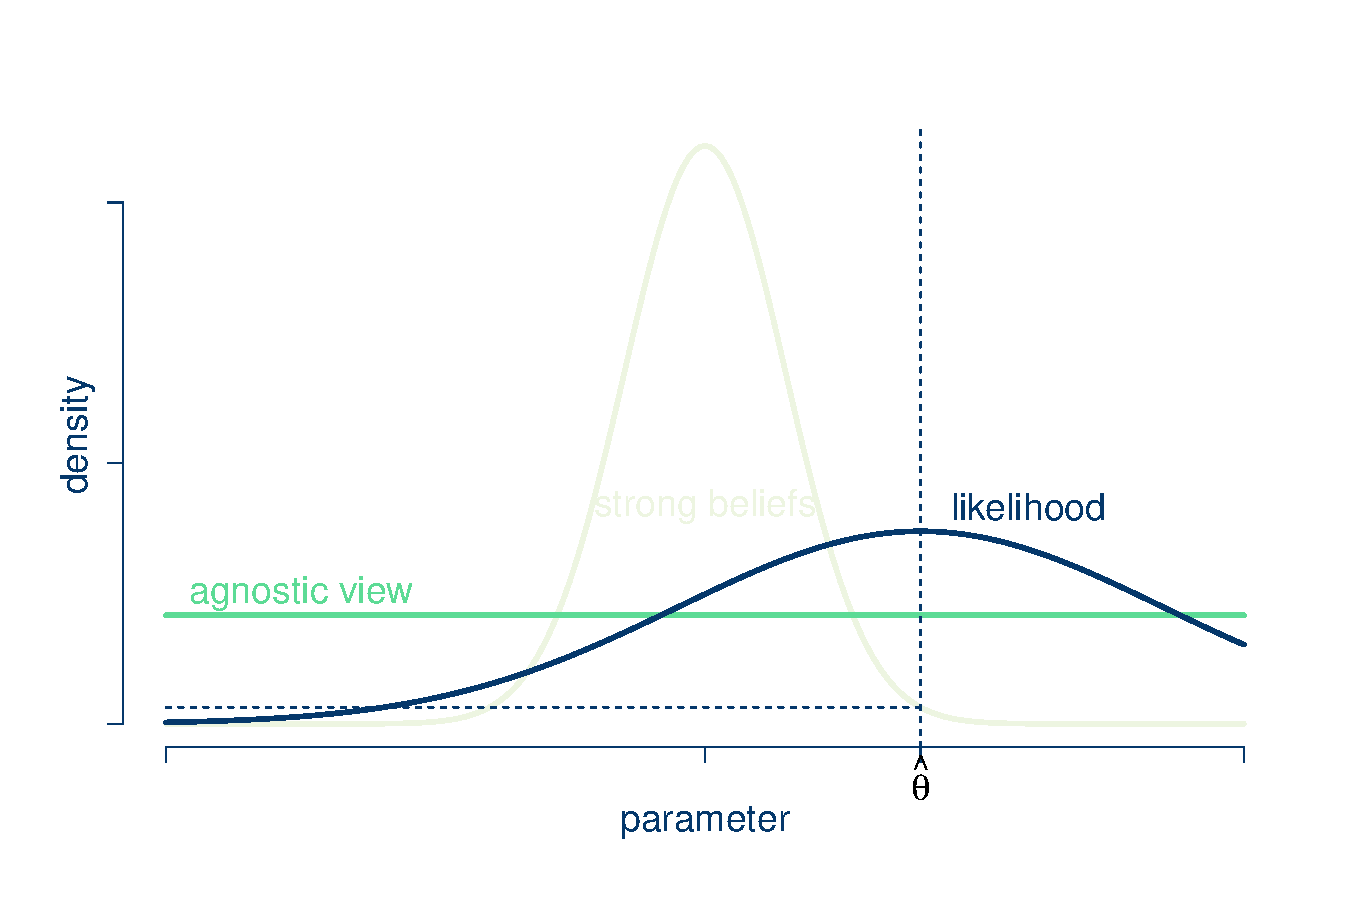
\includegraphics[scale=0.4]{grphs/priors.pdf}
\end{center}

{\color{mcxs1}A prior distribution formalises researcher's beliefs regarding the parameters of the model before seeing the data.}

\end{frame}
}


{\setbeamercolor{background canvas}{bg=mcxs1}
\begin{frame}
\frametitle{Prior distribution}

\centering
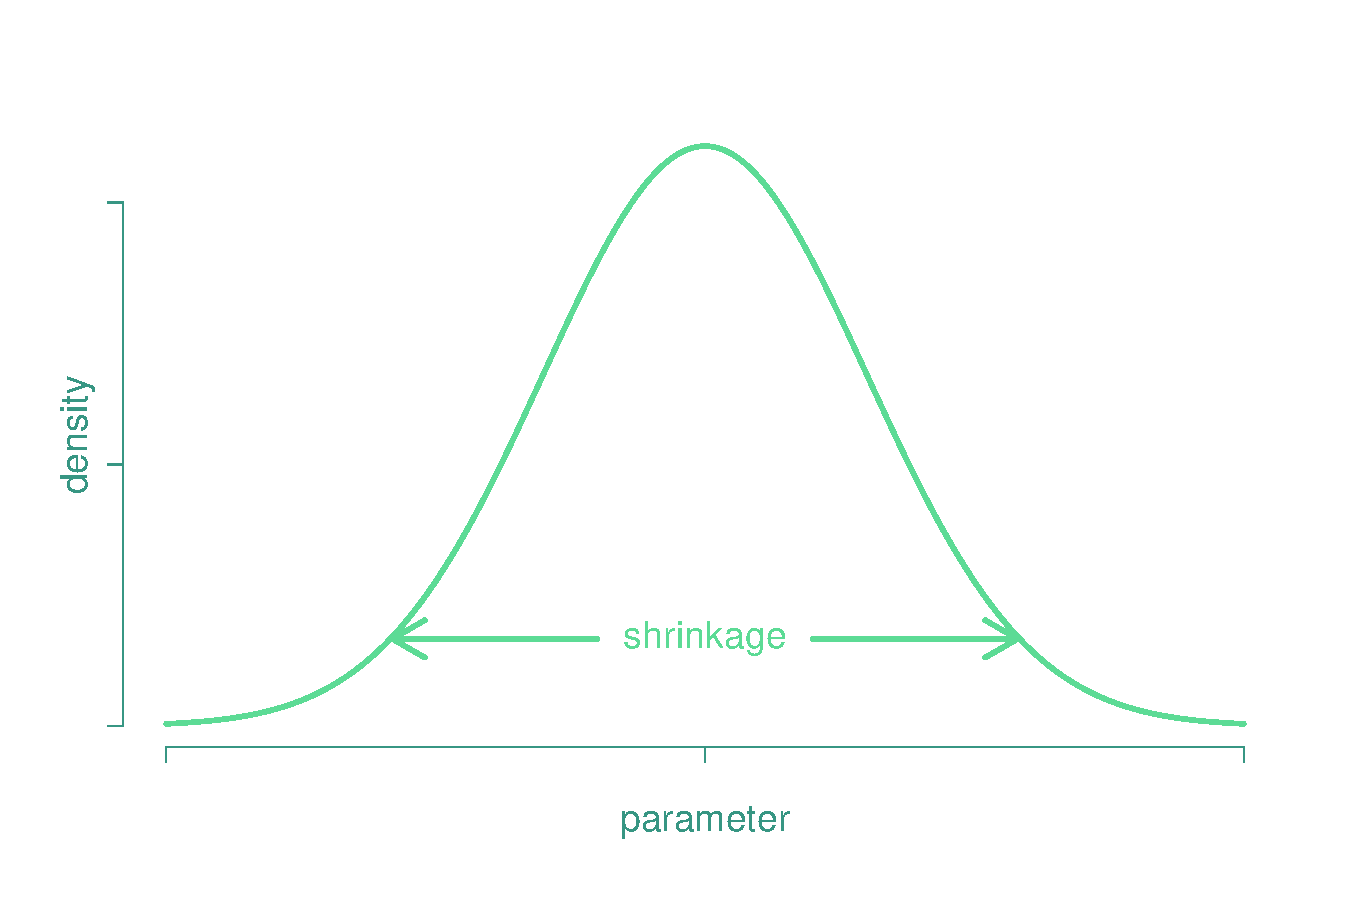
\includegraphics[scale=0.45]{grphs/shrinkage.pdf}

\end{frame}
}




\begin{frame}
\frametitle{Natural-conjugate prior distribution}
\small
{\color{mcxs2}A natural-conjugate prior distribution is of the same form as the distribution of the parameters implied by the likelihood function.}
\begin{align*}
p\left({\color{mcxs3}\beta}, {\color{mcxs3}\sigma^2}\right) &= p\left({\color{mcxs3}\beta}|{\color{mcxs3}\sigma^2}\right)p\left({\color{mcxs3}\sigma^2}\right)\\[1ex]
p\left({\color{mcxs3}\beta}|{\color{mcxs3}\sigma^2}\right)&=\mathcal{N}\left( \underline{\beta}, {\color{mcxs3}\sigma^2}\underline{\sigma}_{\beta}^2 \right)\\
p\left({\color{mcxs3}\sigma^2}\right)&=\mathcal{IG}2(\underline{s},\underline{\nu})
\end{align*}
{\color{mcxs2}Then,} $({\color{mcxs3}\beta,\sigma^2})$ {\color{mcxs2}follow a priori a normal inverse gamma 2 distribution:}
$$ p\left({\color{mcxs3}\beta,\sigma^2}\right)=\mathcal{NIG}2_N\left(\underline{\beta}, \underline{\sigma}_{\beta}^2, \underline{s},\underline{\nu} \right) $$


\bigskip\textbf{pdf.}\footnotesize
\begin{equation*} 
\mathcal{NIG}2_{(N=1)}\left(\underline{\beta}, \underline{\sigma}_{\beta}^2, \underline{s},\underline{\nu} \right) \propto \left({\color{mcxs3}\sigma^2}\right)^{-\frac{\underline{\nu}+3}{2}}\exp\left\{ -\frac{1}{2}\frac{1}{{\color{mcxs3}\sigma^2}}\frac{1}{\underline{\sigma}_{\beta}^2}({\color{mcxs3}\beta}-\underline{\beta})'({\color{mcxs3}\beta}-\underline{\beta}) \right\}
\exp\left\{ -\frac{1}{2}\frac{\underline{s}}{{\color{mcxs3}\sigma^2}} \right\}
\end{equation*} 
\end{frame}












{\setbeamercolor{background canvas}{bg=mcxs2}
\begin{frame}

\begin{adjustwidth}{-0.5cm}{0cm}
%\FlushLeft
\vspace{8.3cm}\Large
\textbf{{\color{mcxs1}Posterior} {\color{mcxs3}distribution}}
\end{adjustwidth}

\end{frame}
}





\begin{frame}
\frametitle{Posterior distribution}


\begin{align*}
p\left( {\color{mcxs3}\beta,\sigma^2}|Y,X \right) &\propto L\left( Y|X,{\color{mcxs3}\beta,\sigma^2} \right)p\left( {\color{mcxs3}\beta,\sigma^2} \right)\\
&= L\left( Y|X,{\color{mcxs3}\beta,\sigma^2} \right)p\left( {\color{mcxs3}\beta}|{\color{mcxs3}\sigma^2} \right)p\left( {\color{mcxs3}\sigma^2} \right)
\end{align*}

\bigskip\textbf{Kernel of posterior distribution.}\scriptsize
\begin{align*}
p\left( {\color{mcxs3}\beta,\sigma^2}|Y,X \right) \propto &
\left( {\color{mcxs3}\sigma^2} \right)^{-\frac{T}{2}}\exp\left\{ -\frac{1}{2}\frac{1}{\color{mcxs3}\sigma^2} ({\color{mcxs3}\beta} - \hat\beta)'X'X ({\color{mcxs3}\beta} - \hat\beta) \right\} \exp\left\{ -\frac{1}{2}\frac{1}{\color{mcxs3}\sigma^2}  (Y-\hat\beta X)'(Y-\hat\beta X) \right\}\\
&\times \left({\color{mcxs3}\sigma^2}\right)^{-\frac{\underline{\nu}+3}{2}}\exp\left\{ -\frac{1}{2}\frac{1}{{\color{mcxs3}\sigma^2}}\frac{1}{\underline{\sigma}_{\beta}^2}({\color{mcxs3}\beta}-\underline{\beta})'({\color{mcxs3}\beta}-\underline{\beta}) \right\}
\exp\left\{ -\frac{1}{2}\frac{\underline{s}}{{\color{mcxs3}\sigma^2}} \right\}
%&=\left( {\color{mcxs3}\sigma^2} \right)^{-\frac{\underline{\nu}+T+3}{2}}\exp\left\{ -\frac{1}{2}\frac{1}{\color{mcxs3}\sigma^2} 
%\left[ \frac{1}{\underline{\sigma}_{\beta}^2}({\color{mcxs3}\beta}-\underline{\beta})'({\color{mcxs3}\beta}-\underline{\beta}) + ({\color{mcxs3}\beta} - \hat\beta)'X'X ({\color{mcxs3}\beta} - \hat\beta)\right] \right\}\\
%&\quad\times  \exp\left\{ -\frac{1}{2}\frac{1}{\color{mcxs3}\sigma^2} \left[ \underline{s} + (Y-\hat\beta X)'(Y-\hat\beta X) \right] \right\}
\end{align*}

\end{frame}





\begin{frame}
\frametitle{Posterior distribution}


\textbf{Kernel of posterior distribution.}\\ \scriptsize
\begin{align*}
p\left( {\color{mcxs3}\beta,\sigma^2}|Y,X \right) \propto 
\left( {\color{mcxs3}\sigma^2} \right)^{-\frac{\underline{\nu}+T+3}{2}} &\exp\left\{ -\frac{1}{2}\frac{1}{\color{mcxs3}\sigma^2}
\left[ \frac{1}{\underline{\sigma}_{\beta}^2}({\color{mcxs3}\beta}-\underline{\beta})'({\color{mcxs3}\beta}-\underline{\beta}) + ({\color{mcxs3}\beta} - \hat\beta)'X'X ({\color{mcxs3}\beta} - \hat\beta)\right.\right.\\
&\qquad +   \left.\left. \underline{s} + (Y-\hat\beta X)'(Y-\hat\beta X) \right] \right\}
\end{align*}

\bigskip\normalsize{\color{mcxs2}After derivations, the expression in the square parentheses can be shown to have the following form:}\scriptsize
\begin{multline*} 
\frac{1}{\underline{\sigma}_{\beta}^2}({\color{mcxs3}\beta}-\underline{\beta})'({\color{mcxs3}\beta}-\underline{\beta}) + ({\color{mcxs3}\beta} - \hat\beta)'X'X ({\color{mcxs3}\beta} - \hat\beta) + \underline{s} + (Y-\hat\beta X)'(Y-\hat\beta X)\\
= \overline{\sigma}_{\beta}^{-2}({\color{mcxs3}\beta}-\overline{\beta})'({\color{mcxs3}\beta}-\overline{\beta}) + \underline{s} + \underline{\beta}^2 \underline{\sigma}_{\beta}^{-2} - \overline{\beta}^2 \overline{\sigma}_{\beta}^{-2}  + Y'Y 
\end{multline*} 
\normalsize{\color{mcxs2}where expressions for} $\overline{\beta}$ \normalsize{\color{mcxs2}and} $\overline{\sigma}_{\beta}^{2}$ \normalsize{\color{mcxs2}are given on the next slides.}

\end{frame}




\begin{frame}
\frametitle{Posterior distribution}

{\color{mcxs2}After plugging in the expression, the kernel of the posterior distribution takes the form of:}
\small
\begin{equation*} 
p\left( {\color{mcxs3}\beta,\sigma^2}|Y,X \right) \propto  \left({\color{mcxs3}\sigma^2}\right)^{-\frac{\overline{\nu}+3}{2}}\exp\left\{ -\frac{1}{2}\frac{1}{{\color{mcxs3}\sigma^2}}\frac{1}{\overline{\sigma}_{\beta}^2}({\color{mcxs3}\beta}-\overline{\beta})'({\color{mcxs3}\beta}-\overline{\beta}) \right\}
\exp\left\{ -\frac{1}{2}\frac{\overline{s}}{{\color{mcxs3}\sigma^2}} \right\}
\end{equation*} 

\bigskip\normalsize{\color{mcxs2}in which we recognize the kernel of the normal inverse gamma 2 distribution.}

\end{frame}




\begin{frame}
\frametitle{Posterior distribution}

\begin{align*} 
p\left( {\color{mcxs3}\beta,\sigma^2}|Y,X \right) &= \mathcal{NIG}2_{(N=1)}\left(\overline{\beta}, \overline{\sigma}_{\beta}^2, \overline{s},\overline{\nu} \right)\\[1ex]
\overline{\sigma}_{\beta}^2 &= \left( \underline{\sigma}_{\beta}^{-2} + X'X \right)^{-1} \\
\overline{\beta} &= \overline{\sigma}_{\beta}^2\left( \underline{\sigma}_{\beta}^{-2}\underline{\beta} + X'Y \right) \\ 
\overline{s} &= \underline{s} + \underline{\sigma}_{\beta}^{-2}\underline{\beta}^2 - \overline{\sigma}_{\beta}^{-2}\overline{\beta}^2 + Y'Y \\
\overline{\nu} &= \underline{\nu} + T
\end{align*} 

\end{frame}




\begin{frame}
\frametitle{Posterior distribution}

\textbf{The posterior mean of $\beta$.}
\begin{align*}
\overline{\beta} &= {\color{mcxs2}\overline{\sigma}_{\beta}^2}\left( {\color{mcxs2}\underline{\sigma}_{\beta}^{-2}}\underline{\beta} + X'Y \right) \\[2ex]
&= {\color{mcxs2}\overline{\sigma}_{\beta}^2 \underline{\sigma}_{\beta}^{-2}} \underline{\beta} + {\color{mcxs2}\overline{\sigma}_{\beta}^2 X'X} (X'X)^{-1}X'Y  \\[2ex]
&= {\color{mcxs2}\frac{\underline{\sigma}_{\beta}^{-2}}{ \underline{\sigma}_{\beta}^{-2} + X'X }} \underline{\beta} + {\color{mcxs2}\frac{X'X}{ \underline{\sigma}_{\beta}^{-2} + X'X }} \hat\beta \\[2ex]
&= {\color{mcxs2}\omega} \underline{\beta} + {\color{mcxs2}(1-\omega)}\hat\beta \\ 
\end{align*}
{\color{mcxs2}The posterior mean of} $\beta$ {\color{mcxs2}is the weighted average between the prior mean} $\underline{\beta}$ {\color{mcxs2}and the MLE} $\hat\beta$.
\end{frame}





\begin{frame}
\frametitle{Posterior distribution}

\small
\begin{align*}
\overline{\beta} &= {\color{mcxs2}\frac{\underline{\sigma}_{\beta}^{-2}}{ \underline{\sigma}_{\beta}^{-2} + X'X }} \underline{\beta} + {\color{mcxs2}\frac{X'X}{ \underline{\sigma}_{\beta}^{-2} + X'X }} \hat\beta \\[1ex]
&= {\color{mcxs2}\frac{\frac{\underline{\sigma}_{\beta}^{-2}}{T}}{ \frac{\underline{\sigma}_{\beta}^{-2}}{T} + \frac{X'X}{T} }} \underline{\beta} + {\color{mcxs2}\frac{\frac{X'X}{T}}{ \frac{\underline{\sigma}_{\beta}^{-2}}{T} + \frac{X'X}{T} }} \hat\beta
\end{align*}
\normalsize\textbf{Limits.}\small
\begin{description}
\item[$\lim_{T\rightarrow\infty}\frac{\underline{\sigma}_{\beta}^{-2}}{T} = 0 $] -- as $\underline{\sigma}_{\beta}^{-2}$ is a constant
\item[$\lim_{T\rightarrow\infty}\frac{X'X}{T} = \sigma_X^2$] -- $\sigma_X^2$ is the second non-central moment of $X$
\end{description}

\bigskip\normalsize\textbf{The posterior mean of $\beta$ when $T\rightarrow \infty$.}
$$ \lim_{T\rightarrow\infty}\overline{\beta} = \hat\beta $$
\end{frame}






\begin{frame}

\centering
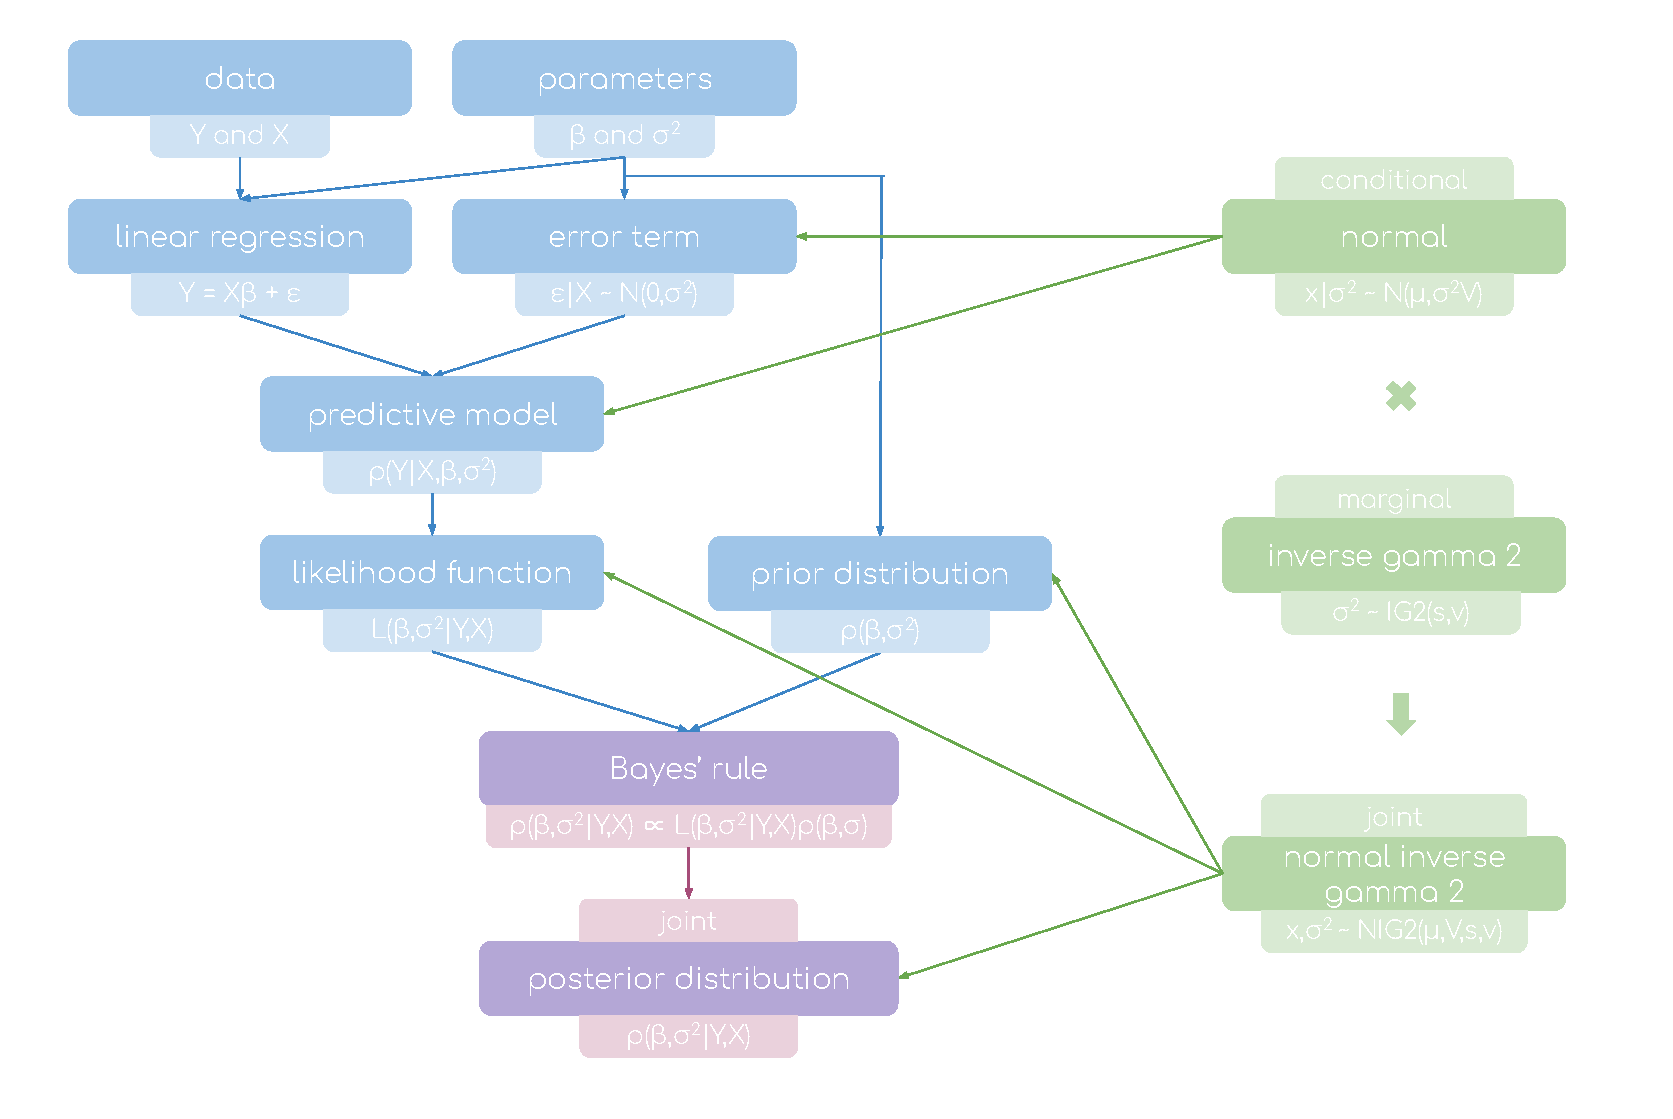
\includegraphics[scale=0.45, trim= 1.8cm 2cm 2cm 0.5cm]{grphs/03conceptmap.pdf}

\end{frame}





{\setbeamercolor{background canvas}{bg=mcxs1}
\begin{frame}{Bayesian estimation}

\begin{description}
\item[{\color{mcxs3}For a linear Gaussian regression:}] {\color{mcxs1}.}

\bigskip\item[{\color{mcxs3}Likelihood function}] {\color{mcxs2}has a form of a Normal inverse gamma~2 distribution for the parameters of the model}

\smallskip\item[{\color{mcxs3}Normal inverse gamma 2 distribution}] {\color{mcxs2}for the parameters is the naturally-conjugate prior distribution leading to...}

\smallskip\item[{\color{mcxs3}Normal inverse gamma 2}] {\color{mcxs2}posterior distribution}

\smallskip\item[{\color{mcxs3}Asymptotically}] {\color{mcxs2}Bayesian estimation converges to the MLE}
\end{description}

\end{frame}
}



%\begin{frame}
%
%
%\includegraphics[scale=0.15]{OnBayesGrave.jpeg}
%\includegraphics[scale=0.15, angle=90]{OnGaussGrave.jpg}
%
%\end{frame}




\end{document} 